\chapter{Introducción}
	
	La escasez de agua aumenta día con día, afectando a más del \qty{40}{\percent} de la población mundial \cite{pnud_objetivo_nodate}. Según datos de la \acrfull{wri} en 2019 globalmente más de 1000 millones de personas vivían en regiones de escasez de agua y para el 2025 este número podría crecer a 3500 millones, siendo las principales causas de esta escasez: la contaminación de cuerpos acuosos, sequías agravadas por la emergencia climática y el uso descontrolado de agua, de pequeña escala en hogares sin buenas prácticas para el cuidado del agua como a escala industrial.
	
	Este problema es innegable y por ello la \acrfull{onu} contempló como sexto objetivo en los \acrfull{ods} el acceso a agua limpia y saneamiento. Estos objetivos pertenecientes a la Agenda 2030 proponen 8 puntos estratégicos para afrontar esta situación, de los cuales, me gustaría resaltar el objetivo 6.a, pues propone una estrategia para abordar la problemática y propone medidas para aminorar este problema.
	
	\begin{displayquote}[][.]
		De aquí a 2030, ampliar la cooperación internacional y el apoyo prestado a los países en desarrollo para la creación de capacidad en actividades y programas relativos al agua y el saneamiento, como los de captación de agua, \textbf{\gls{desalinizacion}}, uso eficiente de los recursos hídricos, tratamiento de aguas residuales, reciclado y tecnologías de reutilización \cite{naciones_unidas_sustainable_nodate}
	\end{displayquote}

	En aras de aportar a esta meta, el presente trabajo propone un sistema para la \gls{desalinizacion_termica} por destilación solar buscando un mejor rendimiento a través del uso de concentradores solares; a lo largo del texto se revisa literatura que encamina la metodología a seguir para lograr la desalinización de agua que asemeje las condiciones de vida marina obtenida artificialmente disolviendo las sales contenidas en los paquetes de sal para acuario.
	
	\section{Antecedentes}

	\subsection{Historia de la energía solar}
		
		El primer registro del uso de concentradores para capturar la energía del sol data del año 212 a.C. por el famoso griego Arquímedes quien usó esta potente energía para defender a Siracusa de una flota romana durante la segunda guerra púnica, la leyenda cuenta que se usaron los escudos de bronce de los guerreros para concentrar los rayos del sol en la madera de los barcos enemigos y así incendiarlos. Aunque no queda registro histórico fiable de esta leyenda, el Dr. Ioannis Sakkas, logró recrear el escenario y en sólo cuestión de minutos, tenía un galeón romano ardiendo \cite{africa_archimedes_1975}.
		
		No fue sino hasta el siglo XVIII que los concentradores solares volvieron a tener aplicación, época donde se construyeron numerosos hornos solares capaces de derretir hierro, cobre y otros metales, siendo uno de los más famosos el diseñado por Antoine Lavoisier el cual alcanzó una increíble temperatura de \SI{1750}{\degreeCelsius}. Récord de temperatura alcanzada por estas técnicas durante poco más del 1 siglo \cite{kalogirou_solar_2004}. Posteriormente otros ilustres personajes como August Mouchot y Abel Pifre continuaron con el diseño de \glspl{colector_solar} para impulsar máquinas de vapor.
		
		En 1839 Becquerel descubrió el efecto fotovoltaico en el selenio, pero no fue sino hasta 1883 que se crea la primera celda solar con una eficiencia de \qtyrange{1}{2}{\percent}; a pesar de estos hechos, la primera vez que se observa y describe el efecto foto eléctrico es hasta 1887 por el físico alemán Heinrich Hertz. 
		
		Teniendo en cuenta que la energía solar a partir de ese momento empezó a tener un gran interés de estudio, la~\cref{table:historia-energia-solar} recopila brevemente hechos destacados de los próximos dos siglos.
		
		\begin{longtblr}[
			caption = {Resumen del avance de la energía solar durante los siglos XX y XXI},
			label = {table:historia-energia-solar},
			remark{Referencias} = {Tabla construida con base en \cites{cassini_explicacion_2008}{kalogirou_solar_2004}{bretado_de_los_rios_aplicacion_2017}{garcia_garrido_guitecnica_2012}{grupo_jab_historia_2018}{ojeda-duran_historia_2018}}
		]{
			colspec = {c X[l]},
			hlines,
			vlines,
			row{odd} = {bg=tablerow},
			row{1} = {
				bg = tabletitle,
				fg=white,
				font =  \large\bfseries
			},
			rowhead = 1,
			rows={m}
		}
			
			{Ubicación temporal} & Evento \\ 
			% Table body%
			1905 & Einstein propone la teoría de la luz y resuelve con ella las incógnitas encontradas en el efecto fotoeléctrico. El descubrimiento de la ley que rige este fenómeno le otorgaría en 1922 el Nobel de Física\\
			1912 & Se instaló la planta de bombeo más grande del mundo en Meadi, Egipto, la cual usaba concentradores de cilindro parabólico logrando hasta \qtyrange{37}{45}{\kilo\watt} continuamente por 5 horas diarias, fue detenida en 1915 por el inicio de la primera guerra mundial y el bajo precio de los combustibles fósiles \\
			1956 & Se empiezan a usar las celdas solares de silicio de manera comercial a pequeña escala \\
			1958 & Se lanza el primer satélite que usaba energía solar (Vanguard I) \\
			Década de 1960 & Se popularizó la industria de los calentadores solares de agua residenciales \\
			1974 & EE.UU. crea el \acrfull{nrel}, laboratorio que fue fundamental para el desarrollo de la energía solar en años posteriores \\
			Década de 1980 & Se ponen en funcionamiento las primeras torres solares de manera demostrativa trasladándose al campo industrial en el 2007 \\
			1982 & Se construye el primer parque solar \\
			1981 &  En España se probó un sistema de \SI{500}{\kilo\watt} de la Agencia Internacional de Energía para generación eléctrica usando concentradores parabólicos en la plataforma solar de Almería. \\
			1994 & El \acrshort{nrel} desarrolla celdas fotovoltaicas con hasta un \qty{30}{\percent} de eficiencia de conversión \\
			2013 & Las celdas solares de perovskita se empiezan a estudiar y tienen un gran auge\\
		\end{longtblr}
		
		
	\subsection{Historia de la desalinación}
		
		La~\cref{table:historia_desalinizacion} hace un resumen histórico de la desalinización.
		
		\begin{longtblr}[
			caption = {Breve historia de la desalinización de agua},
			label = {table:historia_desalinizacion},
			remark{Referencias} = {Tabla construida con base en \cites{kalogirou_solar_2004}{kumar_water_2016}{pau_desaladoras_nodate}{aquae_historia_nodate}{modi_influence_2020}{gonzalez_castro_alternativa_2014}}
		]{
			colspec = {c X[l]},
			hlines,
			vlines,
			row{odd} = {bg=tablerowgreen},
			row{1} = {
				bg = tabletitlegreen,
				fg=white,
				font =  \large\bfseries
			},
			rowhead = 1,
			rows={m}
		}
			Ubicación temporal & Evento \\
			%%% table body %%%
			Siglo III a.C. & Aristóteles ideó el primer evaporador de agua conocido y describe que al evaporarse el agua salada y volverse a condensar, el vapor no forma agua salada de nuevo. 
			\\ 
			Siglo I d.C. & Plinio describe algunos métodos para desalinizar el agua.
			\\ 
			Entre el Siglo II y III & Alejandro de Afrodisias describe el procedicimiento para desalinizar agua del mar.
			\\
			1551 & Se registra el primer uso de destiladores solares por alquimistas árabes
			\\
			Siglo XVI & Se vuelve popular el uso de alambiques para desalinizar agua en los barcos que navegaban por el mar.
			\\
			1869 & Mouchot describe la desalinización por destilación térmica y crea el antecedente de la aplicación del uso de la energía térmica del sol para aplicaciones industriales.
			\\
			1870 & Wheeler y Evans patentan por primera vez en la historia un destilador solar, describiendo a gran detalle los fenómenos de condensación y los problemas de corrosión y absorción de calor
			\\
			1872 & Creación de la primera planta desalinizadora industrial ubicada en Chile.
			\\
			1928 & Pasteur reportó el uso de concentradores solares para desalinizar agua contenida en una caldera de cobre
			\\
			Segunda guerra mundial & Los destiladores solares cobraron gran importancia para el abastecimiento de agua de los soldados en el norte de África y en las islas del océano pacífico.
			\\
			1964 & Primera planta desalinizadora en España.
			\\ 
			1959 & Brenton y Reid demuestran la capacidad de un acetato de luminosa para desalinizar agua. A partir de este momento, la desalinización por ósmosis inversa empezó a llamar la atención.
			\\
		\end{longtblr}

		\subsubsection{Destiladores solares}
		
			\begin{tcolorbox}[
				nobeforeafter,
				breakable,
				title={Hallazgos sobre la eficiencia del destilador solar},
				colback=white,
				colframe=lightblue,
				coltitle=black
			]
				En 1973 Cooper \cite{cooper_maximum_1973} (citado en \cite{ranjan_economic_2016}) encontró que la máxima eficiencia experimental y teórica de los destiladores solares de una fase pueden alcanzar hasta un \qty{60}{\percent} y \qty{50}{\percent}. Entre los motivos hallados, Malik {\it et al.} \cite{malik_solar_1982} (citado en \cite{ranjan_economic_2016}) en 1982 describe las mayores pérdidas que encontraron experimentalmente descritas en la~\cref{table:perdidas_malik}.
			\end{tcolorbox}			
			
			\begin{longtblr}[
				caption = {Pérdidas de un destilador solar},
				label = {table:perdidas_malik}
			]{
				colspec = {X c},
				hlines,
				vlines,
				row{odd} = {bg=tablerowgreen},
				row{1} = {
					bg = tabletitlegreen,
					fg=white,
					font =  \large\bfseries
				},
				rowhead = 1,
				rows={m}
			}
				Motivo & Pérdida \\ 
				% Table body%
				Pérdida de calor por radiación desde la superficie del agua salina a la cubierta & \qty{26}{\percent} \\ 
				Pérdida de calor por el reflejo de la luz & \qty{11}{\percent} \\ 
				Pérdida por reevaporación del destilado & \qty{10}{\percent} \\ 
				Pérdida por el calor absorbido por el vidrio & \qty{5}{\percent} \\ 
				Pérdidas por suelo y bordes & \qty{2}{\percent} \\ 
				Otras pérdidas & \qty{7}{\percent}
			\end{longtblr}
			
			\begin{tcolorbox}[
				title={Breve historia de la destilación solar en México \cite{munoz_gutierrez_sobre_nodate}},
				colback=white,
				colframe=lilac,
				coltitle=black
			]
				\begin{itemize}
					\item México impulsó de 1972 a 1976 la instalación de un gran número de destiladores solares de caseta
					\item A fines de 1975 se inicia el grupo IIUNAM, el cual se dedicó a la investigación sobre las aplicaciones de la energía solar, entre ellas la desalación de agua de mar o salobre
					\item En 1980 en La Paz, Baja California Sur, incluyó un destilador solar de múltiple etapa para el cual se suministró el calor con un arreglo de con­centradores solares de canal parabólico
					\item Durante un año a partir de marzo del 2017 se estudió el comportamiento de varios destiladores solares en Hidalgo, pues es un Estado con agua de alta dureza y con alta irradiancia solar
				\end{itemize}
			\end{tcolorbox}
		
		
			A pesar de que la desalinización solar ha sido objeto de estudio desde siglos atrás, la desalinización solar activa se podría decir que es una tecnología mucho más reciente siendo una idea acuñada por Soliman en 1976 \cite[29]{zheng_solar_2017}. A partir de ese entonces, ha ganado interés y se han propuesto numerosos esquemas para reducir las desventajas de la desalinización solar pasiva.
			
			En agosto de 2017 en Perú fue desarrollado y patentado un destilador solar tipo cascada \cite{saettone_preliminary_2017}. Este sistema tiene una eficiencia global de \qty{71.5}{\percent} produciendo en días soleados \SI[sticky-per]{5690}{\cm\tothe{3}\per\m\tothe{2}} al día y en días nublados \SI[sticky-per]{3648}{\cm\tothe{3}\per\m\tothe{2}} por día.
			
%		\subsubsection{Combinación con otros métodos de desaliniación}
%		¿Iría más en marco teórico?
		
%		
%		%Por otra parte, Veolia Water Technologies \cites{veolia_water_technologies_desalacion_2016}{veolia_water_technologies_seawater_nodate} nos explica que las plantas de desalación híbrida ofrecen una de las tecnologías más eficientes combinando la desalación térmica por destilación con la desalación por ósmosis inversa. En la planta de Fujairah 2 su proceso de desalación térmica comprende 12 unidades \acrshort{med} cuya fuente térmica son los vapores de desecho de una planta industrial cercana, haciendo que la replicación de una planta así, se restrinja geográficamente, requiera de la inversión en infraestructura para el transporte de los vapores y la planificación de mantenimiento para evitar que los vapores de desecho (usualmente tóxicos) se liberen y contaminen de manera irreversible el agua.
	\section{Estado del arte}
	
	El trabajo realizado por \cite{kabeel_performance_2022} hace una investigación sobre la mejora de los mecanismos de transferencia de calor de los destiladores solares, donde se estudia el desempeño de un destilador semiesférico con diferentes tipos de aletas cilíndricas proponiendo diseños como el mostrado en la~\cref{fig:solar-finned-distiller}. Para ver la mejora en el rendimiento, el sistema se probó durante tiempos de 12 horas continuas por 3 días y los resultados obtenidos se compararon contra un destilador semiesférico convencional. 	
		
	\begin{figure}[H]
		\centering
		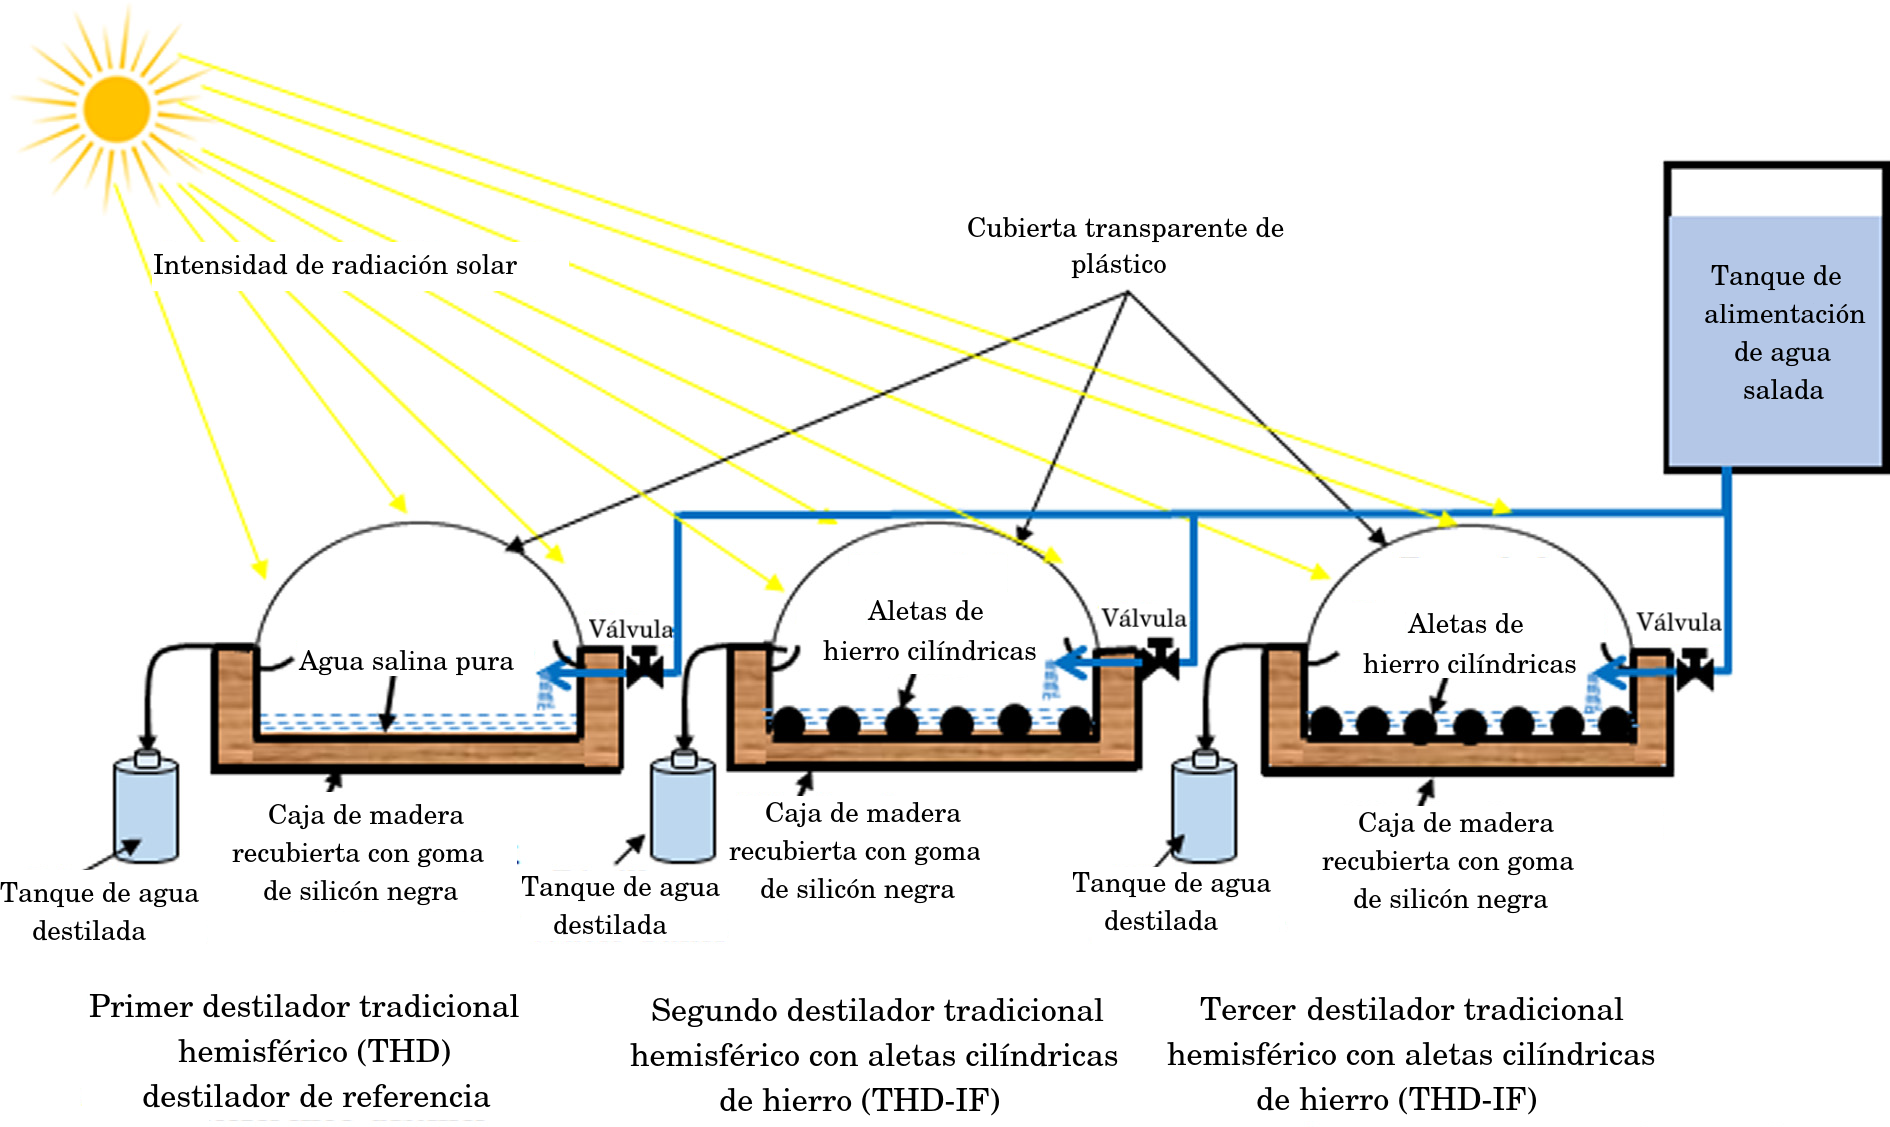
\includegraphics[width=0.8\linewidth, keepaspectratio]{Estado-del-arte/solar-finned-distiller.png}
		\caption{Aletas cilíndricas para mejorar los mecanismos de transferencia de calor de un destilador solar pasivo}
		\floatfoot{Figura obtenida de \cite{kabeel_performance_2022}}
		\label{fig:solar-finned-distiller}
	\end{figure}
	
	De los resultados se observó una mejora de \SI{4.80}{\litre\per\day} del destilador convencional a un promedio de \SI{5.74}{\litre\per\day} del destilador aletado, también se alcanzó una eficiencia de hasta \qty{53.52}{\percent} y se determinó que el sistema tenía una recuperación económica de 24 días.
	
	Jobrane et al. \cite{jobrane_theoretical_2022} propusieton en 2022 un destilador de dos cámaras; se estimó que el costo del agua generada es de 25 euros por cada cien litros de agua, teniendo una producción promedio de \SI{4.03}{\litre\per\m\tothe{2}\day} considerando una potencia recibida promedio de \SI{380}{\watt\per\m\tothe{2}}. Sobre el agua obtenida se realizaron estudios físicos y químicos donde se determinó que poseía buena calidad para beber.
	
	En la~\cref{fig:solar-wick-distiller} se observa la configuración usada; el sistema consta de una cámara de evaporación la cual distribuye el agua bombeada uniformemente sobre una lámina de aluminio AW6060 donde acopla un extractor para forzar la convección del vapor generado hacia la cámara de condensación, donde se reutiliza el calor latente de vaporización para precalentar el agua salobre y a su vez condensar el vapor. Para su alimentación se usó una bomba peristáltica controlada automáticamente y optimizada según el rendimiento visto en el destilador.
	
	\begin{figure}[H]
		\centering
		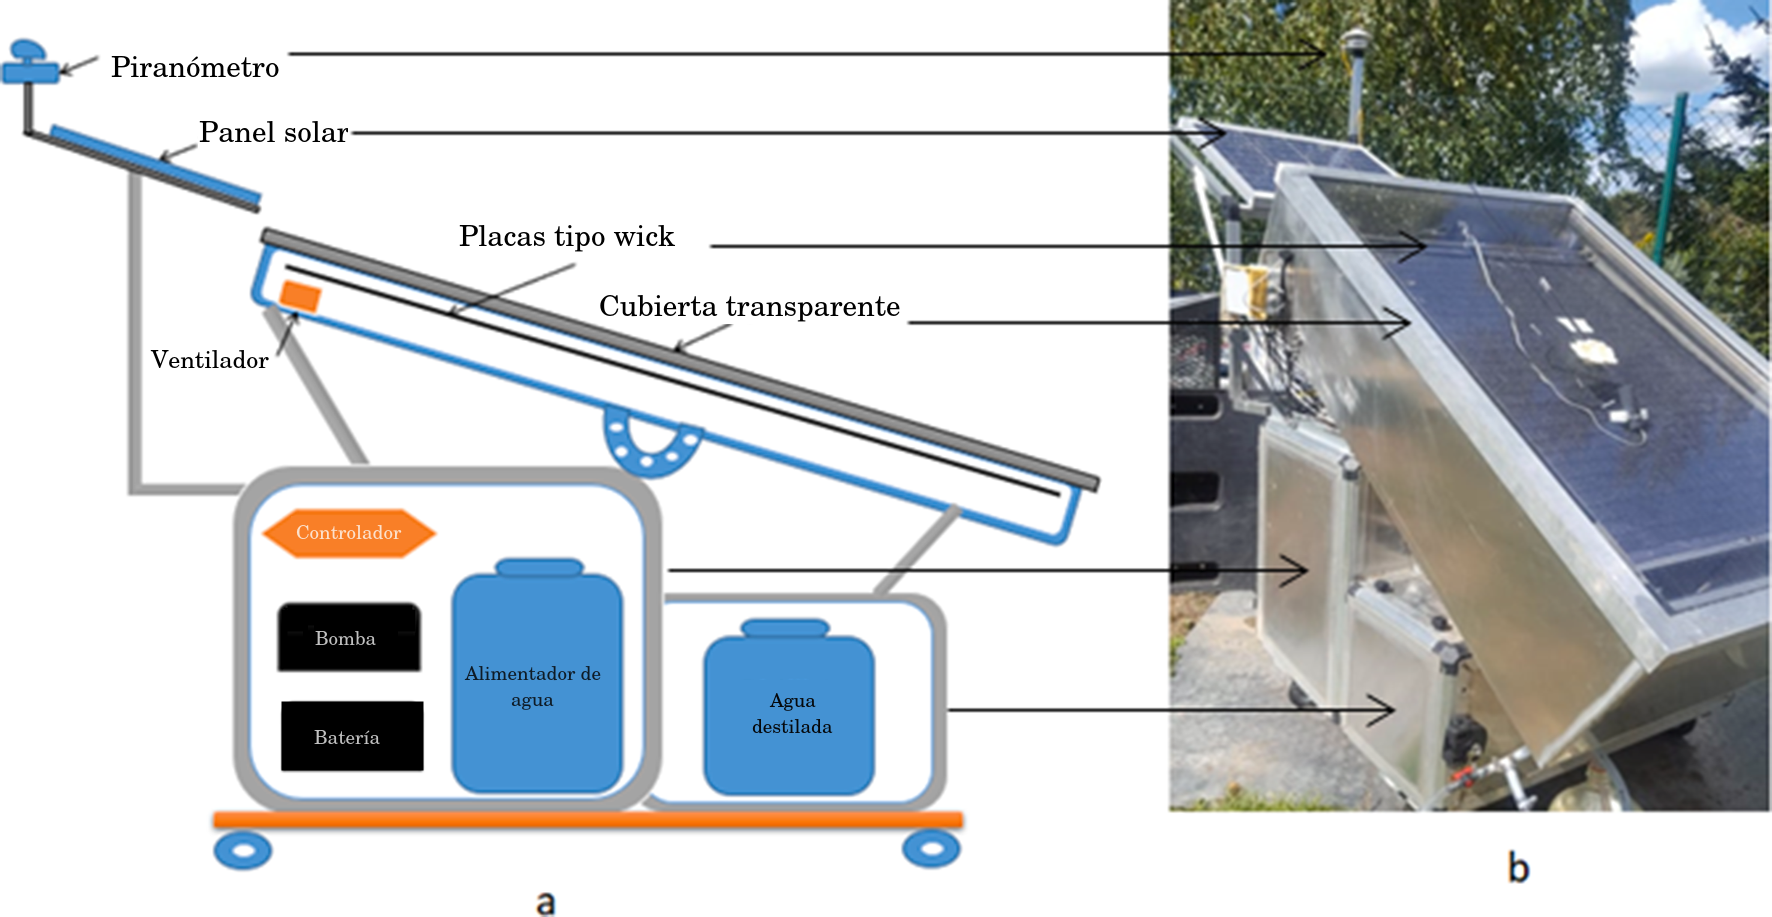
\includegraphics[width=0.8\linewidth, keepaspectratio]{Estado-del-arte/solar-wick-distiller.png}
		\caption{Destilador solar de dos cámaras con ventilador}
		\floatfoot{Figura obtenida de \cite{jobrane_theoretical_2022}}
		\label{fig:solar-wick-distiller}
	\end{figure}
	
	Palomino et al. \cite{palomino-resendiz_design_2018} propusieron un destilador solar híbrido el cual alcanza los \SI{10}{\litre} por día en días soleados con menos de \SI{13}{\gram\per\litre} de sales disueltas. En la \cref{fig:palomino-distiller} se observa el esquema propuesto, el cual se monta sobre una estructura robótica acoplada a un sistema de seguimiento solar y un sistema de control para regular la alimentación del agua. Se observa que este sistema aprovecha tanto la energía solar térmica como la solar fotovoltaica cuyos excedentes son almacenados en baterías.
	
	Este desalinizador totalmente autónomo es potenciado mediante el uso de lentes de Fresnel y un calentador eléctrico. La energía térmica generada por ambos instrumentos es aprovechada dentro de una cámara adiabática de evaporación la cual lleva el vapor generado a un condensador externo.
	
	\begin{figure}[H]
		\centering
		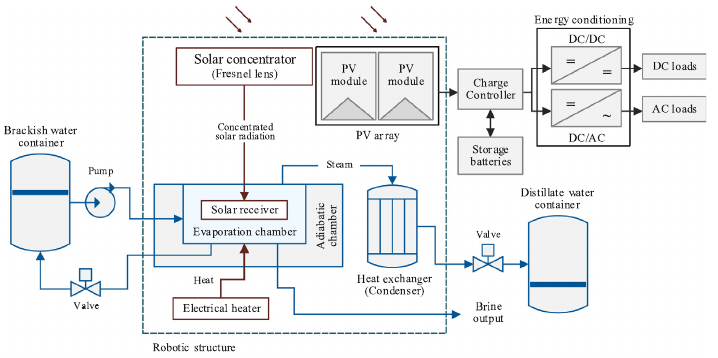
\includegraphics[width=0.8\linewidth, keepaspectratio]{Estado-del-arte/palomino-distiller.png}
		\caption{Destilador solar activo e híbrido con la incorporación de un calentador eléctrico y lentes de concentración.}
		\floatfoot{Figura traducida de \cite{palomino-resendiz_design_2018}}
		\label{fig:palomino-distiller}
	\end{figure}